\documentclass[a4paper,10pt]{report}\input{../0.Préambule/Préambule_cours_prof}\begin{document}

\newpage
\setcounter{chapter}{6}
\chapter{Les nombres relatifs}

\section{Définitions}

\begin{dft}
Un nombre relatif est formé d'un signe $+$ ou $–$ et d'un nombre appelé distance à zéro.
\end{dft}

\begin{ex}
$(+5)$ est un nombre relatif, son signe est $+$ et sa distance à zéro est $5$.

\begin{center}
\begin{tikzpicture}[x=2cm]  
\draw[thick,->] (-1,0) -- (7.5,0);
\foreach \x in {0,+5}
\draw[shift={(\x,0)},color=black] (0pt,6pt) -- (0pt,-6pt) node [below] {\x};
\foreach \x in {-1,1,2,3,4,6,7}	
\draw[shift={(\x,0)},color=black] (0pt,3pt) -- (0pt,-3pt) ;
\end{tikzpicture}
\end{center}

\medskip
\noindent $(-3)$ est un nombre relatif, son signe est $-$ et sa distance à zéro est $3$.

\begin{center}
\begin{tikzpicture}[x=2cm]  
\draw[thick,->] (-5,0) -- (1.5,0);
\foreach \x in {-3,0,1}
\draw[shift={(\x,0)},color=black] (0pt,6pt) -- (0pt,-6pt) node [below] {\x};
\foreach \x in {-5,-4,-2,-1,}	
\draw[shift={(\x,0)},color=black] (0pt,3pt) -- (0pt,-3pt) ;
\end{tikzpicture}
\end{center}
\end{ex}

\begin{dft}
Les nombres comportant un signe $–$ sont appelés les nombres négatifs.

\noindent Les nombres comportant un signe $+$ sont appelés les nombres positifs.
\end{dft}

\begin{rmq}
$0$ n'a pas de signe car il est à la fois positif et négatif.
\end{rmq}

\section{Repérage sur un axe et comparaison}

\begin{dft}
Une droite graduée est une droite qui contient un point nommé Origine, un autre appelé Unité et un sens.
\end{dft}

\begin{ex}

\vspace{1cm}

\begin{center}
\begin{tikzpicture}[x=1.5cm]  
\draw[thick,->] (-5,0) -- (5.5,0);
\foreach \x in {0,1}
\draw[shift={(\x,0)},color=black] (0pt,6pt) -- (0pt,-6pt) node [below] {\x};
\foreach \x in {-5,-4,-3,-2,-1,2,3,4,5}	
\draw[shift={(\x,0)},color=black] (0pt,3pt) -- (0pt,-3pt) ;
\end{tikzpicture}
\end{center}
\end{ex}

\begin{dft}
Sur une droite graduée, chaque point est repéré par un nombre relatif. On dit que ce nombre est l'abscisse de ce point.
\end{dft}

\begin{ex}
\begin{center}
\begin{tikzpicture}[x=1.5cm]  
\draw[thick,->] (-5,0) -- (5.5,0);
\foreach \x in {-2,0,1}
\draw[shift={(\x,0)},color=black] (0pt,6pt) -- (0pt,-6pt) node [below] {\x};
\foreach \x in {-5,-4,-3,-1,2,3,4,5}	
\draw[shift={(\x,0)},color=black] (0pt,3pt) -- (0pt,-3pt) ;
\begin{scriptsize}
\draw[color=blue] (-2,0.5) node {\large{$A$}};
\draw [color=blue] (-2,0)-- ++(-3.5pt,0 pt) -- ++(7.0pt,0 pt) ++(-3.5pt,-3.5pt) -- ++(0 pt,7.0pt);
\draw[color=blue] (4.5,0.5) node {\large{$B$}};
\draw [color=blue] (4.5,0)-- ++(-3.5pt,0 pt) -- ++(7.0pt,0 pt) ++(-3.5pt,-3.5pt) -- ++(0 pt,7.0pt);
\draw[color=blue] (0,0.5) node {\large{$O$}};
\draw [color=blue] (0,0)-- ++(-3.5pt,0 pt) -- ++(7.0pt,0 pt) ++(-3.5pt,-3.5pt) -- ++(0 pt,7.0pt);
\end{scriptsize}
\end{tikzpicture}
\end{center}

\noindent L'abscisse de $A$ est $(-2)$, on le note A$(-2)$. 

\medskip
\noindent $B$ a pour abscisse $+4,5$, on écrit donc $B(+4,5)$.
\end{ex}

\begin{rmq}
L'origine de la droite graduée à pour abscisse 0.
\end{rmq}

\begin{prop}
Entre deux nombres relatifs celui qui est le plus grand est celui qui se trouve le plus à droite sur un axe gradué en conséquence :
\begin{enumerate}
\item[•] Entre deux nombres négatifs, celui qui est le plus grand a la plus petite distance à zéro.
\item[•] Entre deux nombres positifs, celui qui est le plus grand a la plus grande distance à zéro.
\item[•] Entre un nombre positif et un négatif, celui qui est le plus grand est le nombre positif.
\end{enumerate}
\end{prop}

\begin{ex}
\begin{center}
$(+2)<(+12)$ \hspace{3cm} $(-10) <(+14)$ \hspace{3cm} $(-19)< (-12)$
\end{center}

\begin{center}
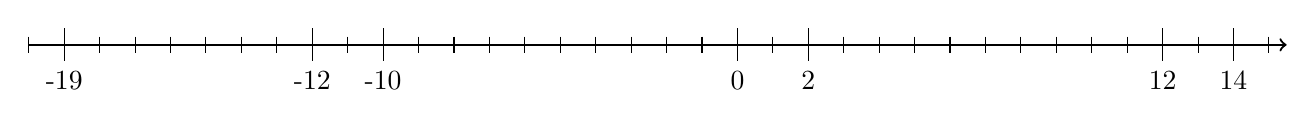
\begin{tikzpicture}[x=0.45cm]  
\draw[thick,->] (-20,0) -- (15.5,0);
\foreach \x in {-19,-12,-10,0,2,12,14}
\draw[shift={(\x,0)},color=black] (0pt,6pt) -- (0pt,-6pt) node [below] {\x};
\foreach \x in {-20,-18,-17,-16,-15,-14,-13,-11,-9,-8,-7,-6,-5,-4,-3,-2,-1,1,3,4,5,6,7,8,9,10,11,13,15}	
\draw[shift={(\x,0)},color=black] (0pt,3pt) -- (0pt,-3pt) ;
\end{tikzpicture}
\end{center}
\end{ex}

\section{Repérage dans un plan}

\vspace{-8mm}
\noindent \begin{minipage}{10cm}
\begin{dft}
Un repère orthogonal du plan est composé de deux droites graduées perpendiculaires et de même origine. 

\medskip
\noindent L'une horizontale est appelée axe des abscisses et l'autre verticale est appelée axe des ordonnées.
\end{dft}
\end{minipage}
\hspace{5mm}
\begin{minipage}{6cm}
\begin{center}
\begin{tikzpicture}[line cap=round,line join=round,>=triangle 45,x=1.0cm,y=1.0cm,scale=0.9]
\begin{axis}[x=1.0cm,y=1.0cm,axis lines=middle,ymajorgrids=false,xmajorgrids=false,
xmin=-3.3,xmax=3.3,ymin=-1.3,ymax=3.3,xtick={-3.0,-2.0,...,3.0},ytick={-1.0,0.0,...,3.0},]
\clip(-3.3,-1.3) rectangle (3.3,3.3);
\end{axis}
\end{tikzpicture}
\end{center}
\end{minipage}

\begin{dft}
Chaque point est repéré par deux nombres appelées coordonnées du point. Le premier nombre est l'abscisse du point et le second l'ordonnée.
\end{dft}

\begin{ex}

\begin{minipage}{9cm}
Ici, $A$ a pour abscisse $-1$ et ordonnées $2$.

\medskip
\noindent On dit que les coordonnées de $A$ sont $(-1; 2)$. 

\medskip
\noindent On note cela :$ A(-1; 2)$

\medskip
\noindent $B$ a pour abscisse $3$ et ordonnées $4$.

\medskip
\noindent On dit que les coordonnées de $B$ sont $(3; 4)$.

\medskip
\noindent On note cela : $B(4; 3)$
\end{minipage}
\begin{minipage}{8cm}
\begin{center}
\begin{tikzpicture}[line cap=round,line join=round,>=triangle 45,x=1.0cm,y=1.0cm,scale=0.8]
\begin{axis}[x=1.0cm,y=1.0cm,axis lines=middle,ymajorgrids=true,xmajorgrids=true,
xmin=-3.3,xmax=4.3,ymin=-1.3,ymax=5.3,xtick={-3.0,-2.0,...,3.0,4.0},ytick={-1.0,0.0,...,5.0},]
\clip(-3.3,-1.3) rectangle (4.3,5.3);
\draw [line width=1.2pt,dash pattern=on 4pt off 4pt] (-1.,2.)-- (-1.,0.);
\draw [line width=1.2pt,dash pattern=on 4pt off 4pt] (-1.,2.)-- (0.,2.);
\draw [line width=1.2pt,dash pattern=on 4pt off 4pt] (3.,4.)-- (0.,4.);
\draw [line width=1.2pt,dash pattern=on 4pt off 4pt] (3.,4.)-- (3.,0.);
\begin{scriptsize}
\draw [color=blue] (-1.,2.)-- ++(-3.5pt,0 pt) -- ++(7.0pt,0 pt) ++(-3.5pt,-3.5pt) -- ++(0 pt,7.0pt);
\draw[color=blue] (-0.86,2.45) node {\large{$A$}};
\draw [color=blue] (3.,4.)-- ++(-3.5pt,0 pt) -- ++(7.0pt,0 pt) ++(-3.5pt,-3.5pt) -- ++(0 pt,7.0pt);
\draw[color=blue] (3.14,4.45) node {\large{$B$}};
\end{scriptsize}
\end{axis}
\end{tikzpicture}
\end{center}
\end{minipage}
\end{ex}

\end{document}